\documentclass{article}
\usepackage{graphics,epsfig}
\def\cG{r_\Gamma}
\def\nn{\nonumber}
\def\beq{\begin{displaymath}}
\def\eeq{\end{displaymath}}
\def\e{\epsilon}
\begin{document}
\begin{center}
{\bf \Large QCDLoop}\\
\vspace{0.3cm}
{\Large R. K. Ellis and G. Zanderighi}\\
\vspace{0.3cm}
December 2007
\end{center}

The f77 library QL, in combination with the library FF, provides
a seamless way of evaluating divergent or finite one-loop scalar
integrals.  We work in the Bjorken-Drell metric so that
$l^2=l_0^2-l_1^2-l_2^2-l_3^2$. \ As illustrated in Fig.~\ref{btbtfig}
the definition of the integrals is as follows
\begin{eqnarray}
&& I^{D}_1(m_1^2)  =
 \frac{\mu^{4-D}}{i \pi^{\frac{D}{2}}\cG}\int d^D l \;
 \frac{1}{(l^2-m_1^2+i\varepsilon)}\,, \nn \\
&& I^{D}_2(p_1^2;m_1^2,m_2^2)  =
 \frac{\mu^{4-D}}{i \pi^{\frac{D}{2}}\cG}\int d^D l \;
 \frac{1}
{(l^2-m_1^2+i\varepsilon)
((l+q_1)^2-m_2^2+i\varepsilon)}\,,\nn \\
&& I^{D}_3(p_1^2,p_2^2,p_3^2;m_1^2,m_2^2,m_3^2)  =
\frac{\mu^{4-D}}{i \pi^{\frac{D}{2}}\cG}
\nn \\
&& \times \int d^D l \;
 \frac{1}
{(l^2-m_1^2+i\varepsilon)
((l+q_1)^2-m_2^2+i\varepsilon)
((l+q_2)^2-m_3^2+i\varepsilon)}\,,\nn \\
&&\nn \\
&&
I^{D}_4(p_1^2,p_2^2,p_3^2,p_4^2;s_{12},s_{23};m_1^2,m_2^2,m_3^2,m_4^2)
= 
\frac{\mu^{4-D}}{i \pi^{\frac{D}{2}}\cG}
\nn \\
&&
\times \int d^D l \;
 \frac{1}
{(l^2-m_1^2+i\varepsilon)
((l+q_1)^2-m_2^2+i\varepsilon)
((l+q_2)^2-m_3^2+i\varepsilon)
((l+q_3)^2-m_4^2+i\varepsilon)}\,, \nn 
\end{eqnarray}
The divergences of the integrals are regulated by dimensional
regularization, $D=4-2 \epsilon$ and we have removed the overall
constant which occurs in $D$-dimensional integrals
\beq
\cG\equiv\frac{\Gamma^2(1-\e)\Gamma(1+\e)}{\Gamma(1-2\e)} = 
\frac{1}{\Gamma(1-\e)} +{\cal O}(\e^3) =
1-\e \gamma+\e^2\Big[\frac{\gamma^2}{2}-\frac{\pi^2}{12}\Big]
+{\cal O}(\e^3)\,.
\nn
\eeq

The numerical code returns the three complex coefficients in the
Laurent series, for any $N$-point integral
\beq
I_N^D = \frac{a_{-2}}{\e^2}+\frac{a_{-1}}{\e^1}+a_0\,,\hspace{.5cm} N\leq 4 \,. 
\nn
\eeq
%
As a first thing one should call the ql-initialization subroutine 
\begin{verbatim}
      subroutine qlinit
\end{verbatim}
which calls the ff-initialization subroutine as well. 

The four scalar integrals, (tadpole, bubble, triangle, box) can then be
evaluated by calling the following four fortran functions.  The
arguments of those four functions are defined as follows,
\begin{verbatim}
      double complex function qlI1(m1,mu2,ep)
      double precision msq,musq
      integer ep
C     mi=m(i)^2 is the square of the mass of the propagator i 
C     mu2 is the square of the scale mu
C     ep=-2,-1,0 chooses the term in the Laurent series.
      .....
\end{verbatim}
\begin{verbatim}
      double complex function qlI2(p1,m1,m2,mu2,ep) 
      double precision p1,m1,m2,mu2
      integer ep
C     p1=psq(1) is the squared four-momentum of the external particle i 
C     mi=m(i)^2, i=1,2 are the squares of the mass of the propagator i 
C     mu2 is the square of the scale mu
C     ep=-2,-1,0 chooses the appropriate term in the Laurent series.
      .....
\end{verbatim}
\begin{verbatim}
      double complex function qlI3(p1,p2,p3,m1,m2,m3,mu2,ep)
      double precision p1,p2,p3,m1,m2,m3,mu
      integer ep
C     pi=p(i)^2, i=1,2,3 are the four-momentum squared of the external lines
C     mi=m(i)^2, i=1,2,3,are the squares of the masses of the internal propagators
C     mu2 is the square of the scale mu
C     ep=-2,-1,0 chooses the term in the Laurent series.
      .....
\end{verbatim}
\begin{verbatim}
      double complex function qlI4(p1,p2,p3,p4,s12,s23,m1,m2,m3,m4,mu2,ep)
      double precision p1,p2,p3,p4,s12,s23,m1,m2,m3,m4,mu2
      integer ep
C     pi=p(i)^2, i=1,2,3,4 are the four-momentum squared of the external lines
C     mi=m(i)^2  i=1,2,3,4 are the squares of the masses of the internal propagators
C     sij=(pi+pj)^2 are external invariants
C     mu2 is the square of the scale mu
C     ep=-2,-1,0 chooses the term in the Laurent series.
      .....
\end{verbatim}

\begin{figure}
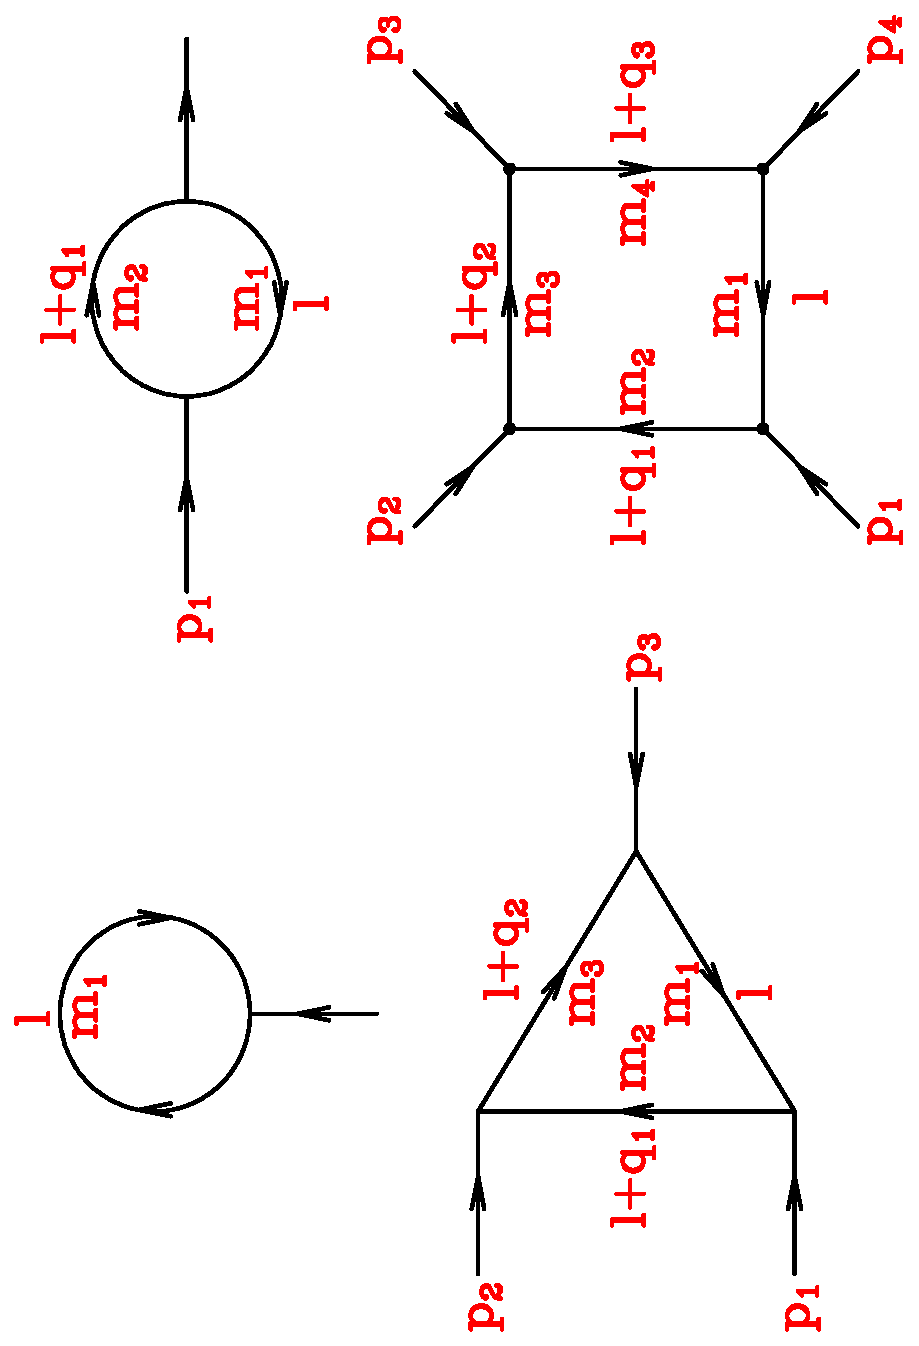
\includegraphics[angle=270,scale=0.55]{tot}
\caption{Tadpole, bubble, triangle and box scalar integrals}
\label{btbtfig} 
\end{figure}

Thus the call to the function
\begin{verbatim}qlI1(10d0,20d0,-1)\end{verbatim} returns the coefficient
of the single pole for the tadpole with internal mass squared $m^2=10$
and $\mu^2=20$.

A full description of the method and analytic results are given in
ref.~\cite{EZ}.  The code relies heavily on the library FF,
ref.~\cite{van Oldenborgh:1990yc}.  In addition, some utility
routines, (the evaluation of complex logarithms and dilogarithms) have
been taken from the looptools distribution, ref.~\cite{Hahn:1998yk}.
The header on the file containing those routines indicates that these
are adapted from routines of Denner.

\begin{thebibliography}{999}
\bibitem{EZ}
R. K. Ellis and G. Zanderighi,
One-loop Scalar integrals for QCD,
Fermilab preprint-PUB-633-T, OUTP-07/16P.

%\cite{van Oldenborgh:1990yc}
\bibitem{van Oldenborgh:1990yc}
  G.~J.~van Oldenborgh,
  %``FF: A Package to evaluate one loop Feynman diagrams,''
  Comput.\ Phys.\ Commun.\  {\bf 66}, 1 (1991).
  %%CITATION = CPHCB,66,1;%%

%\cite{Hahn:1998yk}
\bibitem{Hahn:1998yk}
  T.~Hahn and M.~Perez-Victoria,
  %``Automatized one-loop calculations in four and D dimensions,''
  Comput.\ Phys.\ Commun.\  {\bf 118}, 153 (1999)
  [arXiv:hep-ph/9807565].
  %%CITATION = CPHCB,118,153;%%


\end{thebibliography}

\end{document}
